\section{Tracker controller}

One of the main modules in the reaching controller is represented by the {\tt tracker controller}. The control objective of this specific module consists in directing gaze toward a given target. The input of this module is represented by the target location in the image planes of the right and left eyes; this information is passed by the {\tt target locator} module whose implementation falls outside the scope of this section. The output instead consists in the head motor commands necessary to direct gaze toward the target. 

\subsection{Implementation}

\begin{figure}[tbp]
\centering
\includegraphics[width=120mm]{Figure/SteroImages.jpg}
\caption{Two typical images taken from the two cameras mounted on the eyes of the robot. The attention system gives us the target position on the two image planes. The coordinates of the target on the right image plane will be denoted $u_r$, $v_r$, while on the left image will be denoted $u_l$, $v_l$. The vergence controller task is to move the eyes and the neck in order to keep the target point at the center of the two image planes, i.e. $u_r = v_r = u_l = v_l = 0$.}
\label{Fig:ImagePlane}
\end{figure}

In this section we describe how the tracker has been implemented on James. The crucial aspect concerns the redundancy of the control problem as it has been stated above. In order to state this more clearly, we need to be more rigorous in defining the control task previously described as ``directing gaze toward a given target''. Specifically, let $u_r$ and $v_r$ be the coordinates of the target on the right image plane. Similarly, let $u_l$ and $v_l$ be the coordinates of the target on the left image plane. As it was previously said, the values of $u_r$, $v_r$, $u_l$, $v_l$ will be the output of another module, the {\tt target locator}. Therefore, directing gaze toward the target consists in moving the neck and the eyes so as to obtain $u_r=0$, $v_r=0$, $u_l=0$, $v_l=0$. Let us define the vector $\mathbf x_c = \begin{bmatrix} u_r & v_r & u_l & v_l \end{bmatrix}^\top \in \mathbb R^4$ corresponding to the target location in the image planes. Assuming that the target does not move with respect to the robot, we have that $\mathbf x_c$ can be expressed as a function of the head configuration $\mathbf q_{head} = \begin{bmatrix} \mathbf q_{eyes} & \mathbf q_{neck} \end{bmatrix}^\top \in \mathbb R^6$:
\begin{eqnarray*}
\mathbf x_c = f_{head} (\mathbf q_{head}),
\end{eqnarray*}
where the function $f_{head} : \mathbb R^6 \longrightarrow \mathbb R^4$ depends on the head kinematics. Under suitable assumptions\footnote{The hypothesis is that we do not move the differential tilt, i.e. $\alpha_t^d = 0$ and that the camera optical axis is orthogonal to the pan rotation axis. See also Section \ref{Sec:HeadEyesStructure} for further details.}, we do not need to impose simultaneously the four conditions $u_r=0$, $v_r=0$, $u_l=0$, $v_l=0$ since one of them will be automatically satisfied given that the other three conditions are satisfied\footnote{This fact follows trivially considering that the target moves in a three dimensional space.}.   




Specifically, the target location with respect to the head position is represented by a three dimensional vector 

We implemented a control strategy for verging on a target (blue ball) which has been attached to the robot hand. We assume that there's an attention system on the robot capable of localizing the target on the image plane. 

The strategy we have chosen consists in using a dominant eye (in our case the left eye) to perform a saccade on the desired target and then to follow the dominant eye movement with the neck. This choice is a consequence of the fact that the eyes can make fast movement because of their low inertia. However, their range of movement is small if compared with the neck movement which is characterized by a pretty big range even if with a bigger inertia. This strategy allows us to keep the target always at the center of the image while also allowing a big range of movement for the target itself. Mathematically the above strategy can be implemented as follows:

\begin{eqnarray} 
\left\{ \begin{matrix}
\frac{d \alpha_p^l}{ d t} &=&   K_p u_l\\
\frac{d \theta_y}{ d t} &=&   K_y \alpha_p^l \\
\frac{d \alpha_t^l} {d t} &=&   K_t v_l\\
\frac{d \theta_p} {d t} &=&   K_r \alpha_t^l
\end{matrix} \right.,
\end{eqnarray}
where $\alpha_p^l$ and $\alpha_t^l$ are the pan and tilt positions of the left eye and where $\theta_y$ and $\theta_p$ are the yaw and pitch movement of the neck. This control strategy allows us to asymptotically fixate the target with the left eye ($u_l \rightarrow 0$, $v_l \rightarrow 0$) while also also guaranteeing an asymptotically  straight gaze ($\alpha_p^l \rightarrow 0$, $\alpha_t^l \rightarrow 0$). Another possible control strategy which takes into account the fact that the eye movements anticipate the neck movements is the following:
\begin{eqnarray} \label{Eq:HeadEyeControl}
\left\{ \begin{matrix}
\frac{d \alpha_p^l}{ d t} &=&   K_p u_l\\
\frac{d \theta_y}{ d t} &=&   K_y \alpha_p^l + K_{yp} u_l\\
\frac{d \alpha_t^l} {d t} &=&   K_t v_l\\
\frac{d \theta_p} {d t} &=&   K_r \alpha_t^l + K_{yt} v_l
\end{matrix} \right. .
\end{eqnarray}
In order to verge on the target (i.e. $u_l \rightarrow 0$, $v_l \rightarrow 0$, $u_r \rightarrow 0$, $v_r \rightarrow 0$), we need also to guarantee that $u_r \rightarrow 0$ and $v_r \rightarrow 0$. Assuming that the two cameras are aligned (up to a calibration of the system), we have that $v_r \rightarrow 0$ is automatically implied by $v_l \rightarrow 0$. We are therefore left with guaranteeing that $u_r \rightarrow 0$. This is trivially guaranteed by the following control law:
\begin{eqnarray} \label{Eq:EyeVergenceControl}
\frac{d \alpha_p^r}{ d t} &=&   K_p u_r
\end{eqnarray}
Using the above control strategy (\ref{Eq:HeadEyeControl}) and (\ref{Eq:EyeVergenceControl}),  we obtained the tracking results shown in Figure \ref{Fig:TimeResponse}.

\begin{figure}[tbp]
\centering
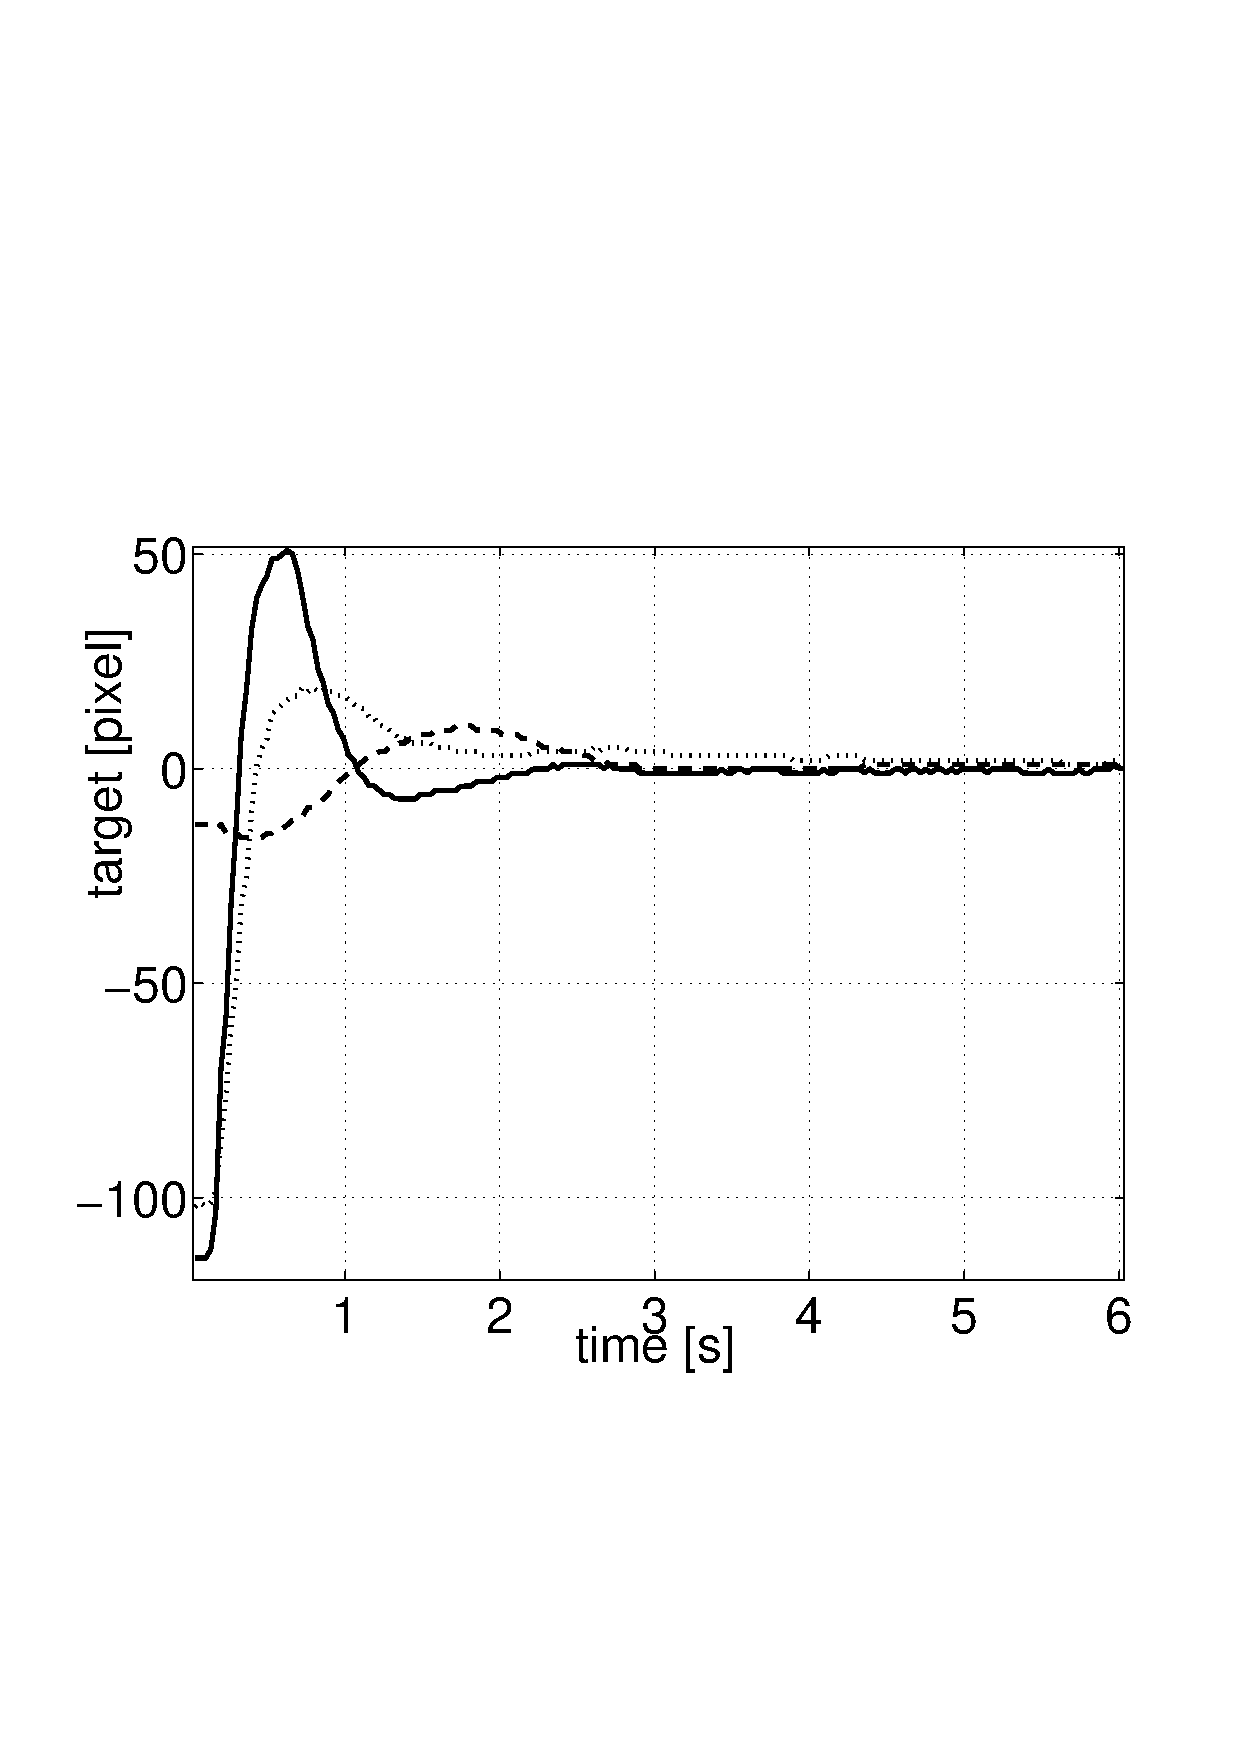
\includegraphics[width=130mm]{Figure/TimeResponseImage.jpg}
\caption{The picture shows the time response of the tracking behavior of the fixation controller. The picture shows that the target is effectively driven to the image center (up to an accuracy of one pixel).}
\label{Fig:TimeResponse}
\end{figure}

\begin{figure}[tbp]
\centering
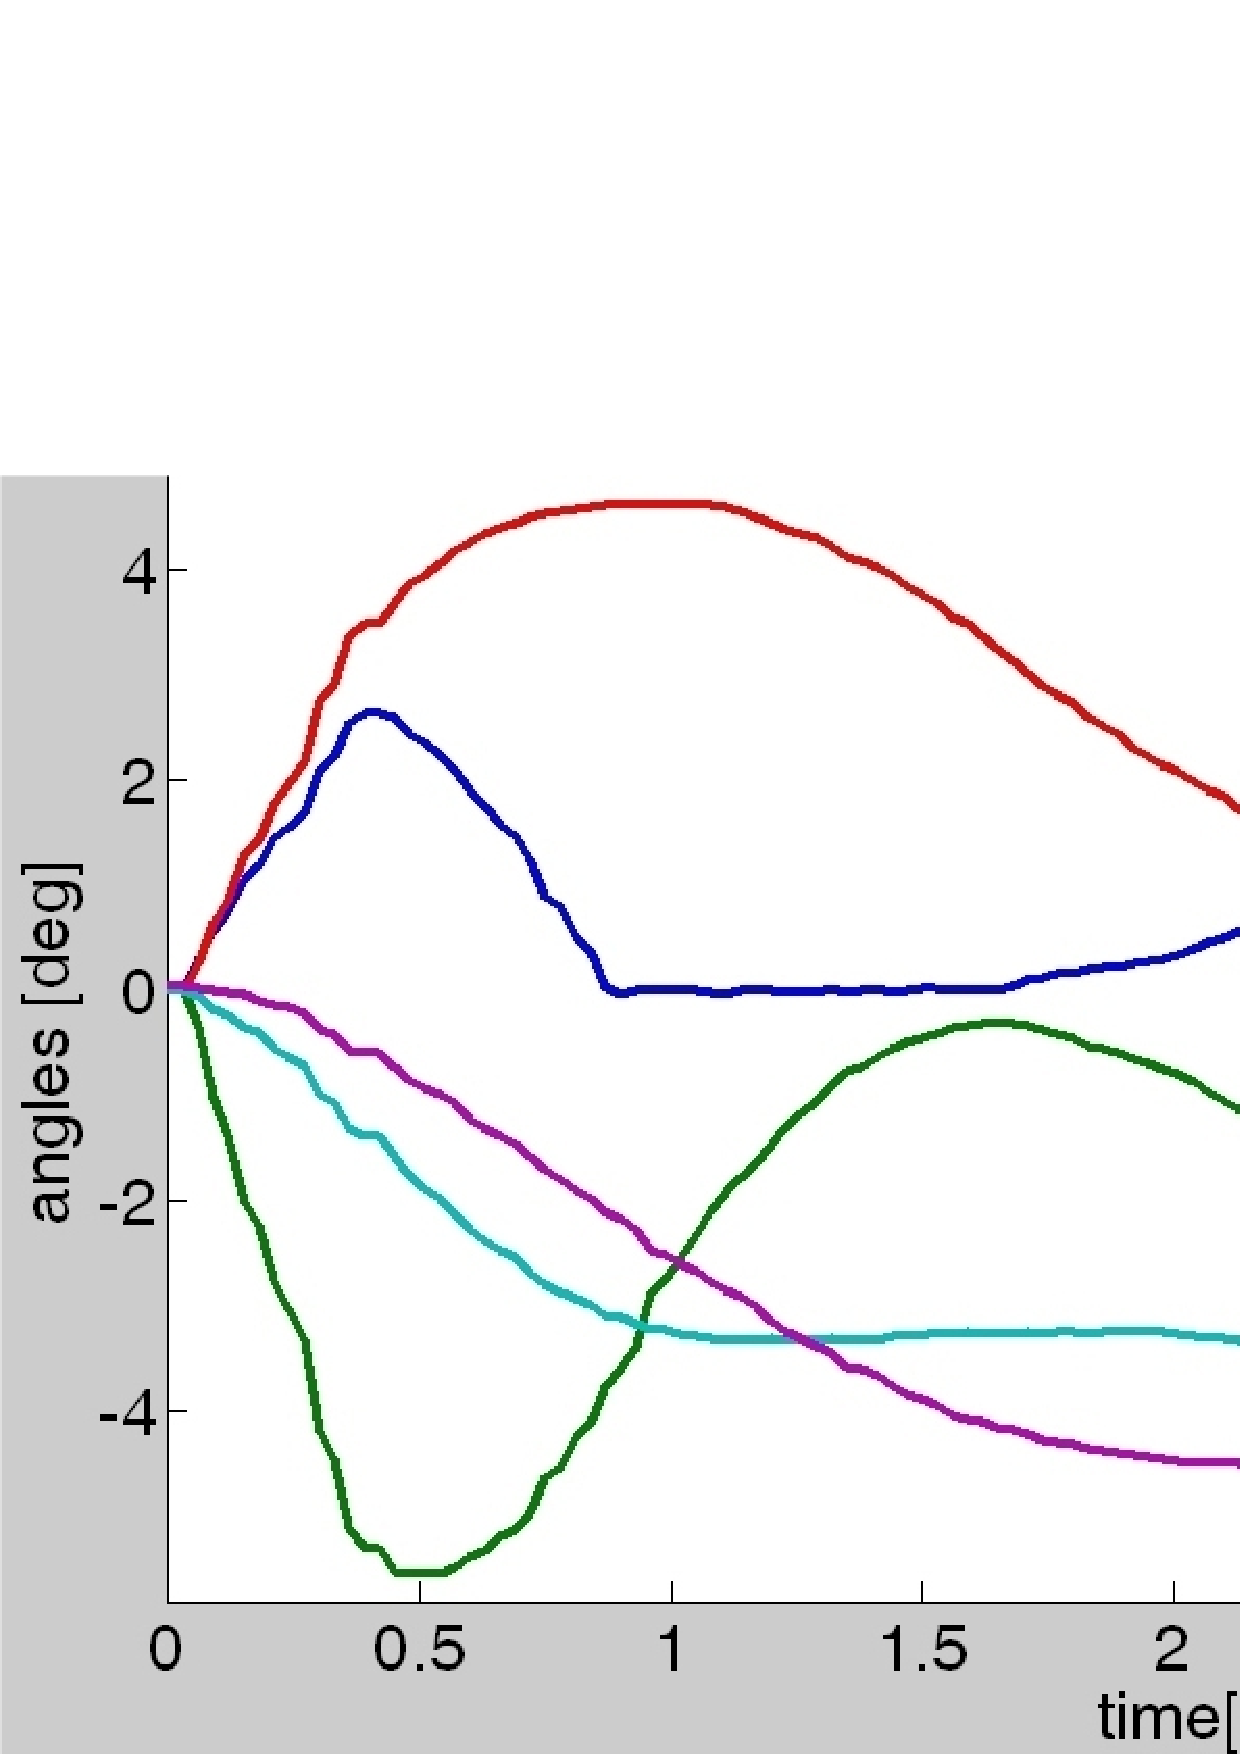
\includegraphics[width=130mm]{Figure/TimeResponseEyesNeck.jpg}
\caption{The picture shows the time response of the tracking behavior of the fixation controller. The picture shows that the dominant eye (left eye) is effectively driven to straight gaze configuration ($\alpha_p^l \rightarrow 0$, $\alpha_t^l \rightarrow 0$ up to an accuracy of one degree). The neck is instead positioned so as to face the target.}
\label{Fig:TimeResponseNeck}
\end{figure}
